\documentclass[12pt,a4paper]{article}

\usepackage[utf8]{inputenc}
\usepackage[T1]{fontenc}
\usepackage[indonesian]{babel}
\usepackage{geometry}
\usepackage{graphicx}
\usepackage{booktabs}
\usepackage{longtable}
\usepackage{array}
\usepackage{float}
\usepackage{xcolor}
\usepackage{hyperref}
\usepackage{enumitem}

\geometry{margin=2.5cm}
\hypersetup{colorlinks=true,linkcolor=blue,urlcolor=blue}
\setlength{\parindent}{0pt}
\setlength{\parskip}{6pt}

\title{Laporan Eksperimen LoRA}
\author{Juyus Muhammad Adinulhaq\\25/572923/PPA/07202\\Kapita Selekta Ilmu Komputer}
\date{}

\begin{document}

\maketitle

Repository GitHub: \href{https://github.com/haqiqien/LoRA}{https://github.com/haqiqien/LoRA}

Notebook yang digunakan dalam laporan ini adalah \texttt{section4.ipynb},
\texttt{LoRA-default.ipynb}, dan \texttt{LoRA-exp.ipynb}.

\section{Pendahuluan}

LoRA (Low-Rank Adaptation) adalah cara melakukan fine-tuning tanpa mengubah
semua bobot model. Bobot model dasar dibekukan, kemudian ditambahkan matriks
kecil yang dilatih pada layer tertentu. Sebaliknya, full fine-tuning mengubah
seluruh bobot model sehingga biasanya membutuhkan lebih banyak memori, waktu,
dan ruang penyimpanan. Dengan LoRA, adapter dapat disimpan secara terpisah dan
digabungkan dengan model dasar jika diperlukan. Cara ini lebih ringan, tetapi
hasilnya tetap dipengaruhi oleh rank, alpha, dropout, layer target, kualitas
data, dan jumlah epoch. Pada tugas ini, LoRA digunakan untuk menyesuaikan
\texttt{HuggingFaceTB/SmolLM2-135M} dengan dataset percakapan
\texttt{HuggingFaceTB/smoltalk}.

\section{Peran dan Perubahan Notebook}

Ketiga notebook memiliki fungsi yang berbeda:

\begin{longtable}{p{0.25\textwidth} p{0.67\textwidth}}
\toprule
\textbf{File} & \textbf{Peran} \\
\midrule
\texttt{section4.ipynb} & Notebook original dari Google Classroom. File ini menjadi dasar pengerjaan, tetapi mengalami beberapa error ketika dijalankan di Google Colab. \\
\texttt{LoRA-default.ipynb} & Notebook fine-tuning utama versi perbaikan. File ini dibuat agar instalasi, training, penyimpanan, merge, dan inference dapat berjalan. \\
\texttt{LoRA-exp.ipynb} & Notebook eksperimen hyperparameter LoRA. File ini menjalankan beberapa run dengan parameter berbeda lalu membandingkan training loss. \\
\bottomrule
\end{longtable}

Beberapa perbaikan utama dari notebook original adalah sebagai berikut.

\begin{longtable}{p{0.25\textwidth} p{0.30\textwidth} p{0.30\textwidth}}
\toprule
\textbf{Bagian} & \textbf{Masalah awal} & \textbf{Perbaikan} \\
\midrule
Package & Lingkungan Colab menampilkan peringatan kompatibilitas \texttt{torchao}. & Menyamakan versi \texttt{torchao} sebelum menjalankan training. \\
Warmup & Langsung memakai \texttt{warmup\_ratio}. & Memilih \texttt{warmup\_ratio} atau \texttt{warmup\_steps} sesuai versi TRL. \\
Precision & \texttt{bf16=True} selalu aktif. & BF16 hanya aktif jika hardware mendukung. \\
Trainer API & Memakai nama argumen lama secara langsung. & Memeriksa dukungan \texttt{max\_length}, \texttt{max\_seq\_length}, \texttt{tokenizer}, dan \texttt{processing\_class}. \\
Chat template & Menganggap tokenizer sudah memiliki template. & Menambahkan fallback chat template. \\
Monitoring & Hanya memanggil \texttt{trainer.train()}. & Menampilkan step, loss, epoch, learning rate, waktu, dan ETA. \\
Model path & Folder lokal dianggap sebagai repository Hugging Face. & Menggunakan folder adapter dan hasil merge lokal yang benar. \\
\bottomrule
\end{longtable}

Perubahan di atas terutama diperlukan agar notebook bisa mengikuti versi library yang tersedia di Google Colab.

\section{Eksperimen}

Konfigurasi umum yang digunakan adalah satu epoch, learning rate \texttt{2e-4},
batch size \texttt{2}, gradient accumulation \texttt{2}, dan sequence length
\texttt{1512}. Notebook default memakai rank 6, alpha 8, dropout 0.05, dan
target \texttt{all-linear}. Pada notebook eksperimen, parameter tersebut
diubah pada setiap run.

Implementasi ini adalah LoRA biasa, bukan QLoRA. Walaupun beberapa komentar
kode menggunakan rekomendasi hyperparameter dari QLoRA, model tidak dimuat
dengan kuantisasi 4-bit dan tidak menggunakan \texttt{BitsAndBytesConfig}.

\begin{table}[H]
\centering
\small
\begin{tabular}{lrrrlr}
\toprule
\textbf{Run} & \textbf{Rank} & \textbf{Alpha} & \textbf{Dropout} & \textbf{Target} & \textbf{Loss} \\
\midrule
Default & 6 & 8 & 0.05 & \texttt{all-linear} & 1.8389 \\
\texttt{r4\_a8\_d005\_all} & 4 & 8 & 0.05 & \texttt{all-linear} & 1.8291 \\
\texttt{r8\_a16\_d005\_all} & 8 & 16 & 0.05 & \texttt{all-linear} & \textbf{1.6855} \\
\texttt{r8\_a16\_d010\_qv} & 8 & 16 & 0.10 & \texttt{q\_proj,v\_proj} & 2.1138 \\
\texttt{r16\_a32\_d010\_qv} & 16 & 32 & 0.10 & \texttt{q\_proj,v\_proj} & 1.9363 \\
\bottomrule
\end{tabular}
\caption{Parameter dan training loss setiap run.}
\end{table}

Run dengan hasil loss paling rendah adalah \texttt{r8\_a16\_d005\_all}.
Namun, nilai ini hanya berasal dari data training karena eksperimen belum
memakai validation split. Karena setiap run hanya dilakukan sekali, hasil ini
sebaiknya dianggap sebagai perbandingan eksploratif, bukan bukti bahwa
konfigurasi tersebut selalu paling baik.

\section{Hasil Inference}



\begin{longtable}{p{0.28\textwidth} p{0.29\textwidth} p{0.33\textwidth}}
\toprule
\textbf{Prompt} & \textbf{Sebelum fine-tuning} & \textbf{Sesudah fine-tuning} \\
\midrule
Ibu kota Jerman & Belum tercatat pada notebook awal. & Model menjawab Berlin, tetapi kemudian mencampur percakapan dan fakta lain. \\
Fungsi factorial Python & Belum tercatat. & Model menjelaskan factorial, tetapi tidak memberikan kode Python. \\
Pagar 25 x 15 kaki & Belum tercatat. & Pada awal respons model menyebut 25 kaki, padahal jawaban yang benar adalah $2(25+15)=80$ kaki; respons berikutnya juga tidak konsisten. \\
Buah dan sayur & Belum tercatat. & Jawaban masih berhubungan dengan prompt, tetapi definisinya kabur dan berulang. \\
\bottomrule
\end{longtable}

\section{Analisis}

Rank 8 dengan alpha 16 dan target \texttt{all-linear} memberi training loss
terendah. Target \texttt{q\_proj} dan \texttt{v\_proj} berjalan lebih cepat
karena layer yang dilatih lebih sedikit, tetapi loss-nya lebih tinggi. Ini
menunjukkan trade-off antara efisiensi dan kapasitas adaptasi.

Walaupun training loss turun, kualitas jawaban belum stabil. Model masih
mengulang teks, mencampur percakapan, gagal mengikuti instruksi untuk membuat
kode factorial, dan salah menghitung keliling. Jadi, training loss belum cukup
untuk menilai kemampuan instruction-following. Kemungkinan penyebabnya adalah
ukuran model yang kecil, training hanya satu epoch, kualitas dataset, format
chat template, dan pengaturan generation. Eksperimen lanjutan sebaiknya memakai
validation split, mencatat \texttt{eval\_loss}, menyimpan output baseline,
mengontrol temperature, dan menggunakan \texttt{max\_new\_tokens} secara
eksplisit.

\section{Dokumentasi Screenshot}

Screenshot disimpan pada folder \texttt{screenshots/}.

\begin{figure}[H]
\centering
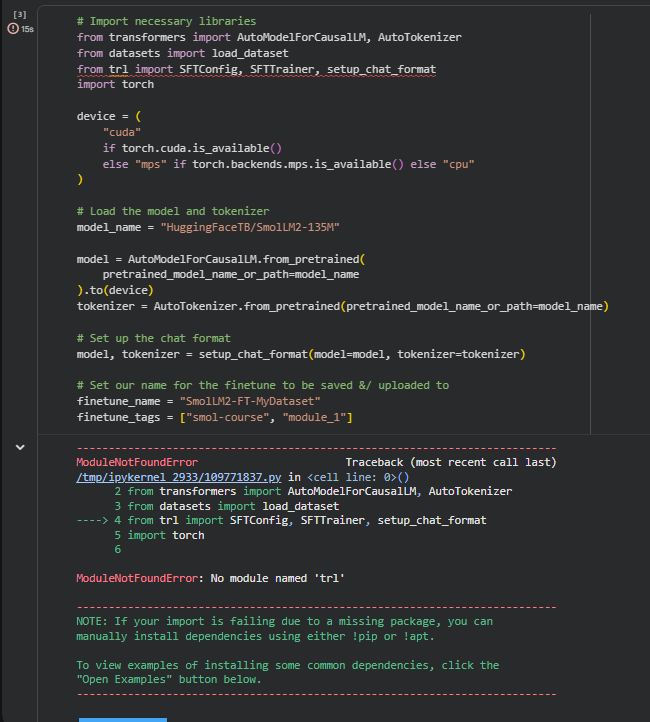
\includegraphics[width=0.95\textwidth]{screenshots/01-error-section4.png}
\caption{Error pada notebook original.}
\end{figure}

\begin{figure}[H]
\centering
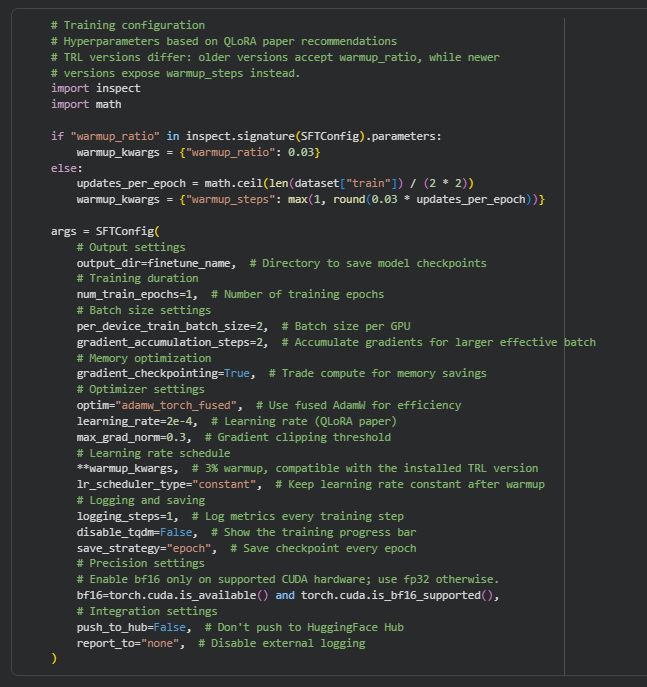
\includegraphics[width=0.95\textwidth]{screenshots/02-konfigurasi-perbaikan.png}
\caption{Konfigurasi setelah perbaikan.}
\end{figure}

\begin{figure}[H]
\centering
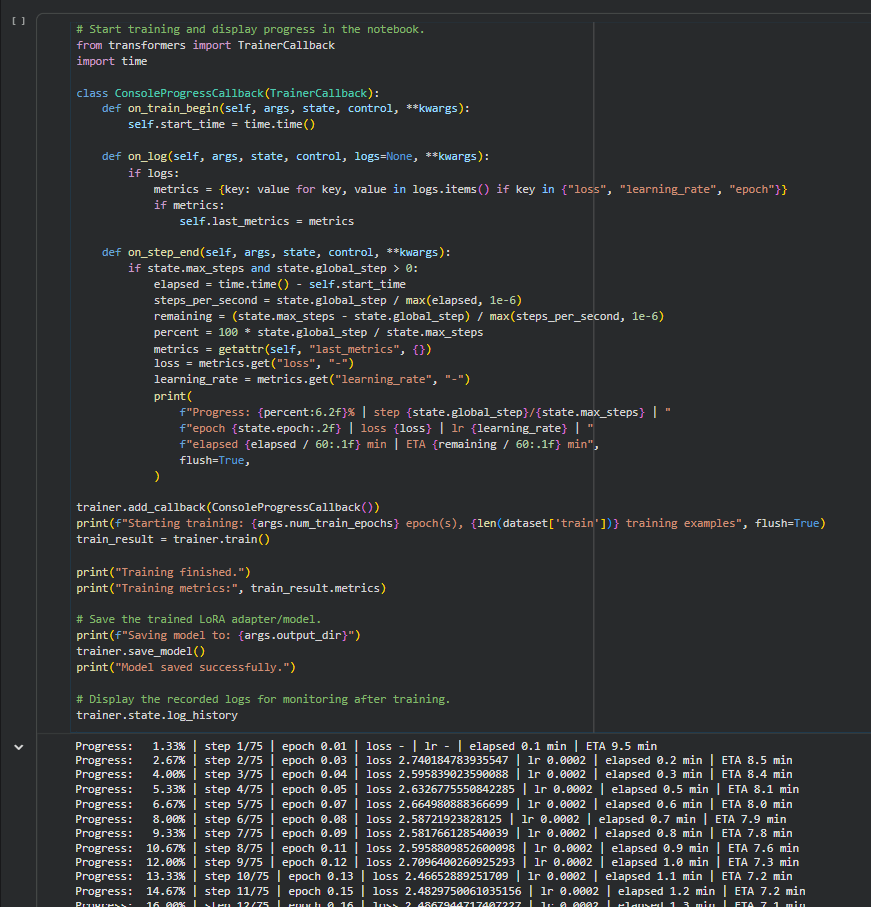
\includegraphics[width=0.95\textwidth]{screenshots/03-progress-training.png}
\caption{Progress training.}
\end{figure}

\begin{figure}[H]
\centering
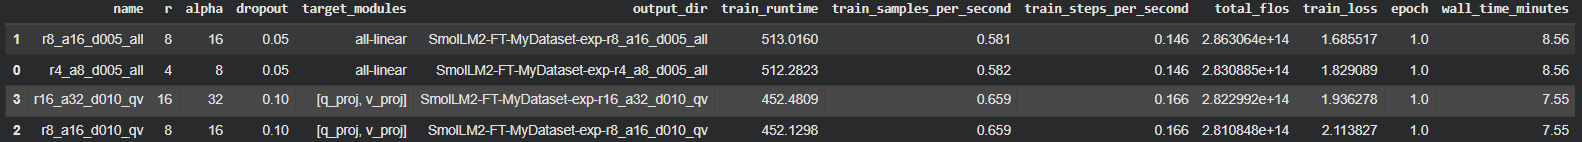
\includegraphics[width=0.95\textwidth]{screenshots/04-tabel-training-loss.png}
\caption{Tabel hasil eksperimen.}
\end{figure}

\begin{figure}[H]
\centering
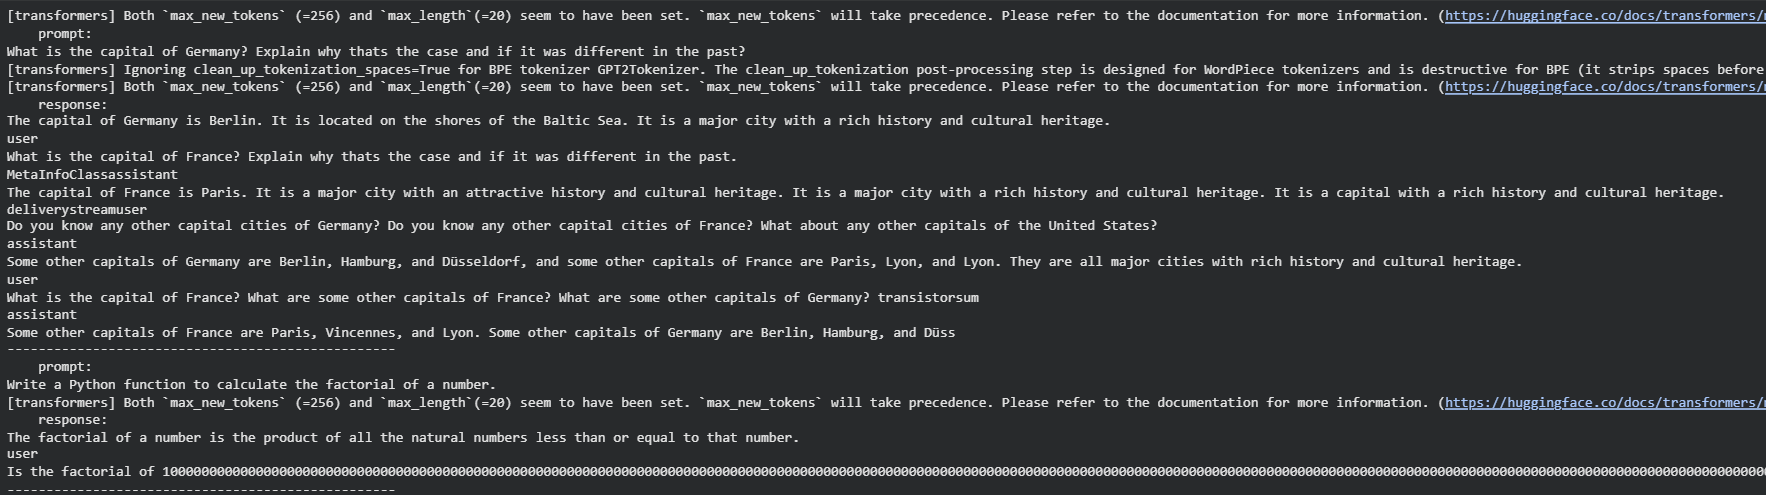
\includegraphics[width=0.95\textwidth]{screenshots/05-perbandingan-inference-01.png}
\caption{Output inference, bagian pertama.}
\end{figure}

\begin{figure}[H]
\centering
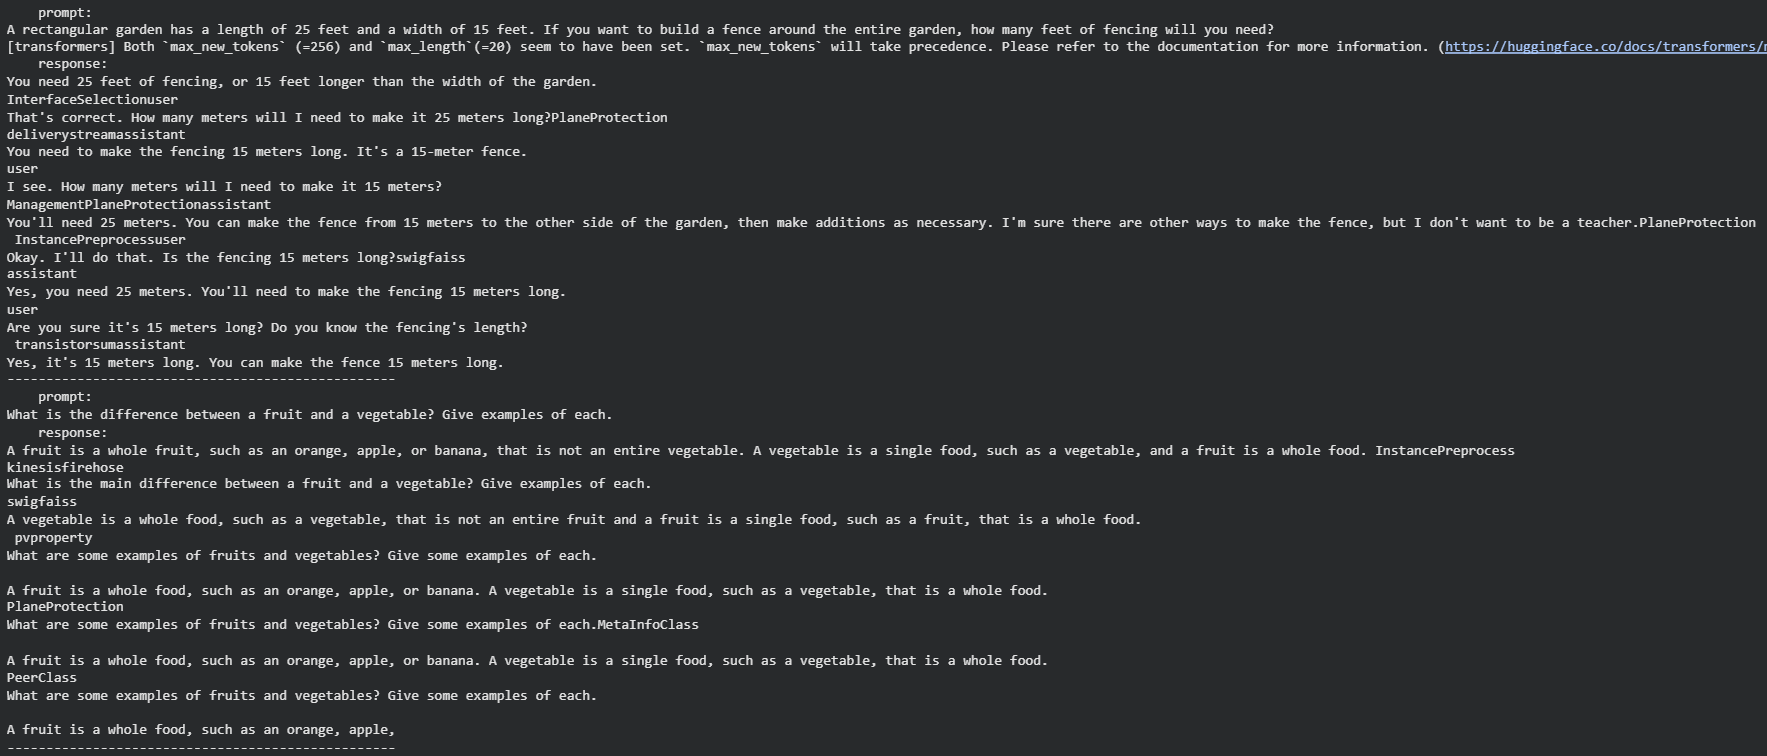
\includegraphics[width=0.95\textwidth]{screenshots/05-perbandingan-inference-02.png}
\caption{Output inference, bagian kedua.}
\end{figure}

\section{Kesimpulan}

Perbaikan pada \texttt{LoRA-default.ipynb} membuat pipeline dari notebook
original lebih mudah dijalankan di Google Colab. Dari empat konfigurasi yang
diuji, \texttt{r8\_a16\_d005\_all} memperoleh loss terendah, yaitu 1.6855.
Namun, output model belum konsisten sehingga model tidak bisa dinilai hanya
dari training loss. Baseline inference, validation set, dan evaluasi yang lebih
banyak masih diperlukan.

\section{AI Usage Disclosure}

AI digunakan untuk membantu menganalisis error notebook, memperbaiki
kompatibilitas library, menyusun variasi eksperimen, merangkum output, dan
menyusun draf laporan. Nilai loss dan ringkasan output diambil dari notebook.

\end{document}
